%% Mixed-Signal Letter, Analog Integrated Circuits and Signal Processing (Springer)
%% Springer Nature LaTeX template (sn-jnl), numbered references (sn-mathphys-num)
%% Compile: pdflatex main; bibtex main; pdflatex main; pdflatex main
\documentclass[pdflatex,sn-mathphys-num,iicol]{sn-jnl}

\usepackage{graphicx}
\usepackage{multirow}
\usepackage{amsmath}
\usepackage{booktabs}
\usepackage{xcolor}
\usepackage[siunitx]{circuitikz}
\usepackage{siunitx}
\sisetup{range-phrase=--, range-units=single}

% placeholder marker for items the authors must complete
\newcommand{\TBD}[1]{\textcolor{red}{[#1]}}

\begin{document}

\title[Multi-input FG floating-body neuron in SKY130]{A multi-input spiking neuron in a single floating-gate, floating-body nMOS transistor: post-layout evidence from the open SKY130 process}

\author*[1]{\fnm{Jos\'e Luis} \sur{Valtierra S\'anchez de la Vega}}\email{\TBD{e-mail}}
\affil*[1]{\orgdiv{Facultad de Ingenier\'ia Mexicali}, \orgname{Universidad Aut\'onoma de Baja California}, \orgaddress{\city{Mexicali}, \state{Baja California}, \country{Mexico}}}

\abstract{Floating-body transistors can fire like neurons because impact ionization charges their body and causes abrupt, hysteretic switching, but published demonstrations rely on measured devices or fitted models. Using only the foundry compact models and layout parasitics of the open SKY130 process, this letter shows that one 5-V nMOS transistor with a floating body and a capacitively coupled floating gate operates as a programmable, multi-input spiking neuron. The stored floating-gate voltage moves the trigger of a static hysteresis from 5.38 to 4.26~V, and with a constant input current the extracted cell fires at 11--210~kHz with 2.5--4.6~pJ per spike inside a current band set by the stored charge. Firing starts at a finite rate (Type~II excitability). Under random input timing, pulses on the control gates act as weighted inputs: the output rate grows with input rate and pulse strength, and two inputs with different coupling capacitors combine as a weighted sum. Trimming the stored charge restores firing across process corners and temperature, and a compact 273-\si{\micro\meter^2} layout fires at 108~kHz.}

\keywords{Spiking neuron, Floating-body MOSFET, Floating gate, Impact ionization, SKY130, Post-layout simulation}

\maketitle

%% ------------------------------------------------------------------
\section{Introduction}\label{sec:intro}

CMOS integrate-and-fire neurons need tens of transistors~\cite{indiveri2011}. Floating-body transistors are a far smaller alternative: holes generated by impact ionization accumulate in an unbiased body, lower the threshold voltage and raise the drain current, producing an abrupt hysteretic jump~\cite{park2018kink}. This has given neurons in partially depleted SOI~\cite{dutta2017} and in bulk transistors whose body is discharged through a second transistor~\cite{pazos2025}. These demonstrations use measured devices or fitted models, and their threshold depends on die-to-die variation~\cite{pazos2025}. Floating gates solve the analogous problem in analog circuits by storing a non-volatile offset on each device~\cite{diorio1996,bhattacharyya2025,hasler2021woset}. This letter merges both mechanisms in one transistor and shows, from the open SKY130 compact models and extracted parasitics alone, that the cell fires with a programmable threshold, sums several capacitively weighted inputs on its own gate, and is trimmed into operation across corners and temperature.

%% ------------------------------------------------------------------
\section{Cell and operating principle}\label{sec:cell}

\begin{figure}[t]
\centering
\resizebox{0.85\linewidth}{!}{% Schematic of the floating-gate floating-body (FGFB) neuron cell
\begin{circuitikz}[american, font=\small]
  % input current and membrane capacitor
  \draw (0,6.8) node[above]{$V_{\mathrm{sup}}$} to[short,o-] (0,6.5)
        to[I, l_=$I_{\mathrm{in}}$] (0,5.0) coordinate (mem);
  \draw (mem) to[C, l_=$C_{\mathrm{mem}}$] (0,2.4) node[ground]{};
  \fill (mem) circle (1.6pt);
  \node[above right] at (mem) {$V_{\mathrm{mem}}$};
  % FGFB transistor M1
  \node[nmos, bulk] (M1) at (6.4,3.2) {};
  \draw (mem) -| (M1.D);
  \draw (M1.S) node[ground]{};
  \node[anchor=west] at ($(M1.D)+(0.2,-0.25)$) {$M_1$};
  % floating-gate network
  \draw (M1.G) -- ++(-1.4,0) coordinate (fg);
  \fill (fg) circle (1.6pt);
  \node[above] at (fg) {FG};
  \draw (fg) to[C, l=$C_{\mathrm{fix}}$] (fg |- 0,1.6) node[ground]{};
  \draw (fg) -- ++(-1.3,0) coordinate (ca);
  \draw (ca) to[C, l=$C_{A}$, -o] (ca |- 0,1.6) node[below]{$V_{A}$};
  \draw (ca) -- ++(-1.3,0) coordinate (cb);
  \draw (cb) to[C, l=$C_{B}$, -o] (cb |- 0,1.6) node[below]{$V_{B}$};
  \fill (ca) circle (1.6pt);
  \node[font=\footnotesize, align=center, anchor=north] at ($(fg)+(0,-2.15)$) {stored charge\\$\Rightarrow V_Q$};
  % body and bulk-control transistor M2
  \draw (M1.bulk) -- ++(1.1,0) coordinate (b);
  \fill (b) circle (1.6pt);
  \node[above] at (b) {body};
  \draw (b) -- ++(0,-0.5) node[nmos, anchor=D, xscale=-1] (M2) {};
  \draw (M2.S) node[ground]{};
  \draw (M2.G) -- ++(0.3,0) node[right]{$V_{G2}$};
  \node[anchor=south] at ($(M2.G)+(0.45,0.05)$) {$M_2$};
  % isolation box
  \draw[dashed, rounded corners] ($(M1.G)+(-0.15,0.95)$) rectangle ($(M1.bulk)+(0.45,-0.95)$);
  \node[font=\scriptsize, align=left, anchor=south west] at ($(M1.G)+(-0.15,0.95)$) {isolated p-well (deep n-well at 5\,V)};
\end{circuitikz}
}
\caption{Floating-gate floating-body neuron. $M_1$ (5-V nMOS) sits in a p-well isolated by a deep n-well at 5~V; its floating gate (FG) couples to inputs $V_A$, $V_B$ and to ground through MIM capacitors and stores a charge represented by $V_Q$. $M_2$ discharges the body with gate bias $V_{G2}$; $I_{\mathrm{in}}$ charges $C_{\mathrm{mem}}$}
\label{fig:schematic}
\end{figure}

In the cell of Fig.~\ref{fig:schematic} the floating-gate voltage is
\begin{equation}
V_{FG} = V_Q + \beta_A V_A + \beta_B V_B + \beta_D V_{\mathrm{mem}},\quad \beta_i = C_i/C_\Sigma ,
\label{eq:vfg}
\end{equation}
where $V_Q$ is the stored charge divided by the total floating-gate capacitance $C_\Sigma$. At high drain voltage the BSIM4 substrate-current term of the foundry model~\cite{bsim4} injects holes into the body; a higher body voltage raises the drain and substrate currents, so the body switches high (clamped by the source junction) once the loop gain exceeds unity. No bipolar or fitted element is added. With $I_{\mathrm{in}}$ charging $C_{\mathrm{mem}}$, the body is the fast variable and the membrane the slow one: $V_{\mathrm{mem}}$ ramps to the trigger, the body switches, $C_{\mathrm{mem}}$ discharges to the release voltage, and $M_2$ resets the body. Because the inputs act through Eq.~\eqref{eq:vfg}, their weights are set by the capacitor ratios $\beta_A$, $\beta_B$.

The cell was drawn in Magic~\cite{magic} with the open\_pdks SKY130A technology~\cite{sky130pdk}. Both transistors are \texttt{nfet\_g5v0d10v5} devices ($W/L=1/0.5$~\si{\micro\meter}). The capacitors are MIM devices: $C_A=C_B=\SI{8.5}{fF}$, $C_{\mathrm{fix}}=\SI{173}{fF}$ and $C_{\mathrm{mem}}=\SI{188}{fF}$ (model values), giving $\beta_{A,B}\approx 0.044$, which matches the \SIrange{77}{82}{mV} floating-gate step measured for a \SI{1.8}{V} input step. The DRC-clean cell measures \qtyproduct{36.3 x 28.1}{\micro\meter}, dominated by the MIM capacitors. Extraction gives \SI{16.8}{fF} on the body (mostly the p-well/deep-n-well junction) and \SI{12.5}{fF} of wiring on the membrane.


\textbf{Methods.} All results use the extracted netlist in ngspice~42~\cite{ngspice} with the open\_pdks SKY130 models (typical corner, \SI{27}{\celsius}, $V_{G2}=\SI{0.5}{V}$ unless stated). The only test-bench elements are an ideal input current source and a \SI{e18}{\ohm} resistor from the floating gate to $V_Q$, which sets the stored charge at the operating point. Halving or doubling the time step changed firing rates by less than 0.01\,\%. \TBD{LLM-use statement, if applicable.}

%% ------------------------------------------------------------------
\section{Results}\label{sec:results}

\begin{figure*}[t]
\centering
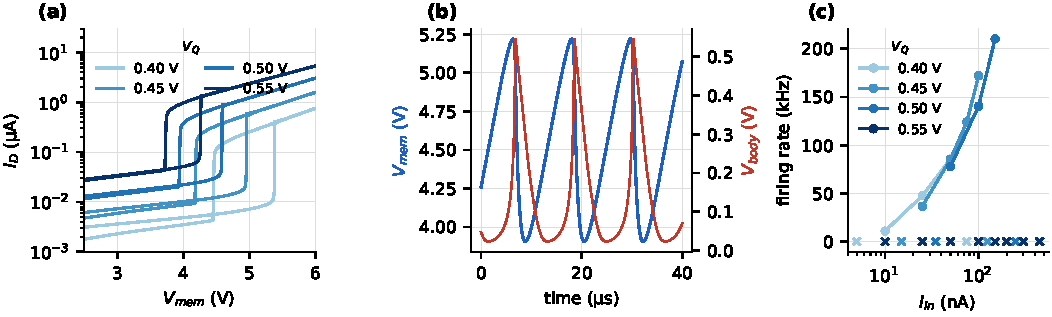
\includegraphics[width=0.88\textwidth]{figs/fig_neuron3.pdf}
\caption{Extracted cell with stock SKY130 models. (a) Quasi-static $I_D$--$V_{\mathrm{mem}}$ loops for four stored-charge values (\SI{2}{ms} ramps). (b) Spiking at $V_Q=\SI{0.45}{V}$, $I_{\mathrm{in}}=\SI{50}{nA}$ (\SI{85.4}{kHz}). (c) Firing rate versus input current; crosses are non-firing points (leak-limited at low current, depolarization block at high current)}
\label{fig:neuron}
\end{figure*}

\subsection{Programmable static hysteresis}
Raising $V_Q$ from 0.40 to \SI{0.55}{V} lowers the trigger voltage from 5.38 to \SI{4.26}{V} and the release voltage from 4.45 to \SI{3.73}{V} (Fig.~\ref{fig:neuron}(a)), a sensitivity of about \SI{7.5}{V/V}. The loop is static: its area changes only from 0.53 to \SI{0.34}{\micro\ampere\volt} when the ramp is slowed 100-fold, from \SI{200}{\micro\second} to \SI{20}{ms}. $V_{G2}$ is a second knob: static loops exist for $V_Q=\SIrange{0.3}{0.7}{V}$ and $V_{G2}=\SIrange{0.3}{0.6}{V}$.


\subsection{Spiking, firing band and excitability class}
With a constant input current the cell fires without clock or reset (Fig.~\ref{fig:neuron}(b)): at $V_Q=\SI{0.45}{V}$ and \SI{50}{nA}, $V_{\mathrm{mem}}$ swings between 3.9 and \SI{5.2}{V} at \SI{85.4}{kHz}. Firing occurs inside a current band (Fig.~\ref{fig:neuron}(c)) bounded below by the leakage of $M_1$ at the trigger and above by a stable high-current state, analogous to depolarization block~\cite{izhikevich2007}. The stored charge shifts the band: about 10--50, 25--100 and \SIrange{50}{150}{nA} for $V_Q=0.40$, 0.45 and \SI{0.50}{V}. Across the bands it fires at 11--\SI{210}{kHz} with 2.5--\SI{4.6}{pJ} per spike ($I_{\mathrm{in}}\langle V_{\mathrm{mem}}\rangle/f$).

Firing begins at a finite rate. At $V_Q=\SI{0.40}{V}$ the cell is silent up to \SI{8}{nA} and fires at \SI{10.9}{kHz} at \SI{10}{nA}. At $V_{G2}=\SI{0.4}{V}$ a sustained oscillation appears just below threshold, growing from 0.14 to \SI{0.58}{V} peak-to-peak between 7.5 and \SI{9}{nA} at a nearly constant \SIrange{15.1}{15.4}{kHz}. This finite-frequency, Hopf-like onset identifies resonator (Type~II) excitability~\cite{izhikevich2007}. Consistent with this, periodic input trains entrain the output at fractions of the input rate ($f_{\mathrm{in}}/3$, $f_{\mathrm{in}}/4$), whereas irregular inputs produce the graded response used below.

\begin{figure*}[t]
\centering
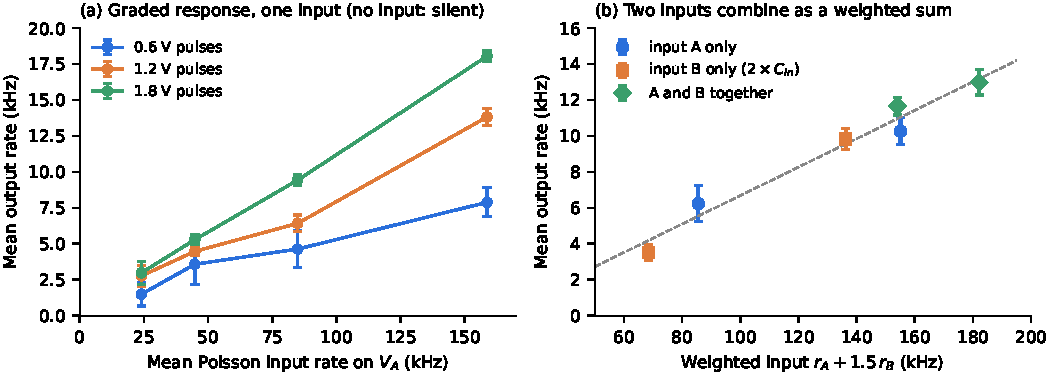
\includegraphics[width=0.76\textwidth]{figs/fig_poisson.pdf}
\caption{Weighted inputs on the floating gate, $V_Q=\SI{0.46}{V}$, $I_{\mathrm{in}}=\SI{20}{nA}$ (silent without input), Poisson trains of \SI{1}{\micro\second} active-low pulses. (a) Output versus input rate on $V_A$ for three pulse amplitudes (mean $\pm$ standard error, seven seeds at most points). (b) Inputs $A$ ($C_A=\SI{8.5}{fF}$) and $B$ ($C_B=\SI{16.3}{fF}$), 0.9-V pulses, six seeds: all single and combined conditions fall on one line against $r_A+1.5\,r_B$}
\label{fig:poisson}
\end{figure*}

\subsection{Weighted inputs}
A falling edge on a control gate lowers $V_{FG}$ by $\beta\,\Delta V$, leaving the membrane above the restored trigger when the pulse ends. Biased just below its firing band ($V_Q=\SI{0.46}{V}$, \SI{20}{nA}), the cell is silent without input and responds to Poisson input trains with a graded rate (Fig.~\ref{fig:poisson}(a)). At about \SI{159}{kHz} input, the output is $7.9\pm1.0$, $13.8\pm0.6$ and $18.1\pm0.4$~kHz for 0.6-, 1.2- and 1.8-V pulses. Since the pulse effect scales with $\beta\,\Delta V$, a coupling capacitor fixes an input's weight. With $C_B$ set to \SI{16.3}{fF} (twice the MIM area) and independent Poisson trains on both inputs, all six single and combined conditions collapse onto one line, $r_{\mathrm{out}}\approx0.079\,(r_A+1.5\,r_B)-\SI{1.2}{kHz}$ (Fig.~\ref{fig:poisson}(b)): the transistor sums its inputs with an effective weight ratio of 1.5 for a 1.9-fold capacitance. The summation thus takes place inside the single device.

\subsection{Robustness, trimming and area}
Of 25 Monte Carlo mismatch samples at $V_Q=\SI{0.45}{V}$, 24 fire ($77.8\pm7.6$~kHz). Process corners and temperature shift the firing window along $V_Q$, and a per-cell trim recovers it: $V_Q=\SIrange{0.15}{0.35}{V}$ for ff, sf and \SI{85}{\celsius}, and $V_Q=\SIrange{0.45}{0.55}{V}$ with $V_{G2}=\SIrange{0.6}{0.7}{V}$ for ss, fs and \SI{-40}{\celsius} (\SIrange{81}{93}{kHz}). The area is set mainly by the MIM capacitors; $C_{\mathrm{mem}}$ scales down to \SI{38}{fF}, about twice the body capacitance, with clean firing after a $V_Q$ retrim. A compact layout with $C_{\mathrm{mem}}=\SI{38}{fF}$ and $C_{\mathrm{fix}}$ stacked over the transistors on the second MIM layer measures \qtyproduct{20.6 x 13.3}{\micro\meter} (\SI{273}{\micro\meter^2}), is DRC-clean, and fires at \SI{108.5}{kHz} ($V_Q=\SI{0.40}{V}$, \SI{20}{nA}).

%% ------------------------------------------------------------------
\section{Discussion}\label{sec:discussion}



Compared with the measured two-transistor floating-body neuron of~\cite{pazos2025}, whose threshold is tuned only by $V_{G2}$, and the six-transistor floating-gate neuron of~\cite{bhattacharyya2025} (350~nm, \SI{2500}{\micro\meter^2}), here one transistor provides the firing nonlinearity, a non-volatile programmable threshold and several weighted inputs in 1020~\si{\micro\meter^2} (273~\si{\micro\meter^2} compact), as predicted by an open PDK without fitted elements. \textbf{Scope.} The SKY130 impact-ionization parameters are extracted with a grounded body, so absolute trigger voltages and currents in the floating-body regime should be confirmed by measurement. Input weights are set at design time by capacitor sizing; floating-gate programming circuitry is outside this study, and the membrane swing (up to \SI{5.9}{V}) calls for a reliability assessment of the 5-V device.

\section{Conclusion}\label{sec:conclusion}
From the open SKY130 compact models and extracted parasitics alone, a single floating-gate, floating-body 5-V nMOS transistor operates as a Type~II spiking neuron whose stored charge programs the threshold and whose control gates sum capacitively weighted inputs; per-cell trimming restores firing across corners and temperature. Measurements of fabricated cells are the next step.

\backmatter

\bmhead{Declarations}
\textbf{Funding:} \TBD{funding statement}. \textbf{Competing interests:} The author has no relevant financial or non-financial interests to disclose. \textbf{Data availability:} Layouts, extracted netlists, test benches and scripts are available at \url{https://github.com/jlvsdlv/fgfb-sky130}. \textbf{Author contributions:} \TBD{CRediT statement}. \TBD{Acknowledgements go on the separate title page.}

\bibliography{refs}

\end{document}
